\section{解析と結果}

\subsection{光量の評価}
今回の解析では、発生光子数ではなく何個のMPPCに光子が入ったかを表すMultiplicityで光量の評価を行った。
図\ref{fig:Multiplicity}にMultiplicityの概念図を示す。

\begin{figure}[htbp]
  \centering
  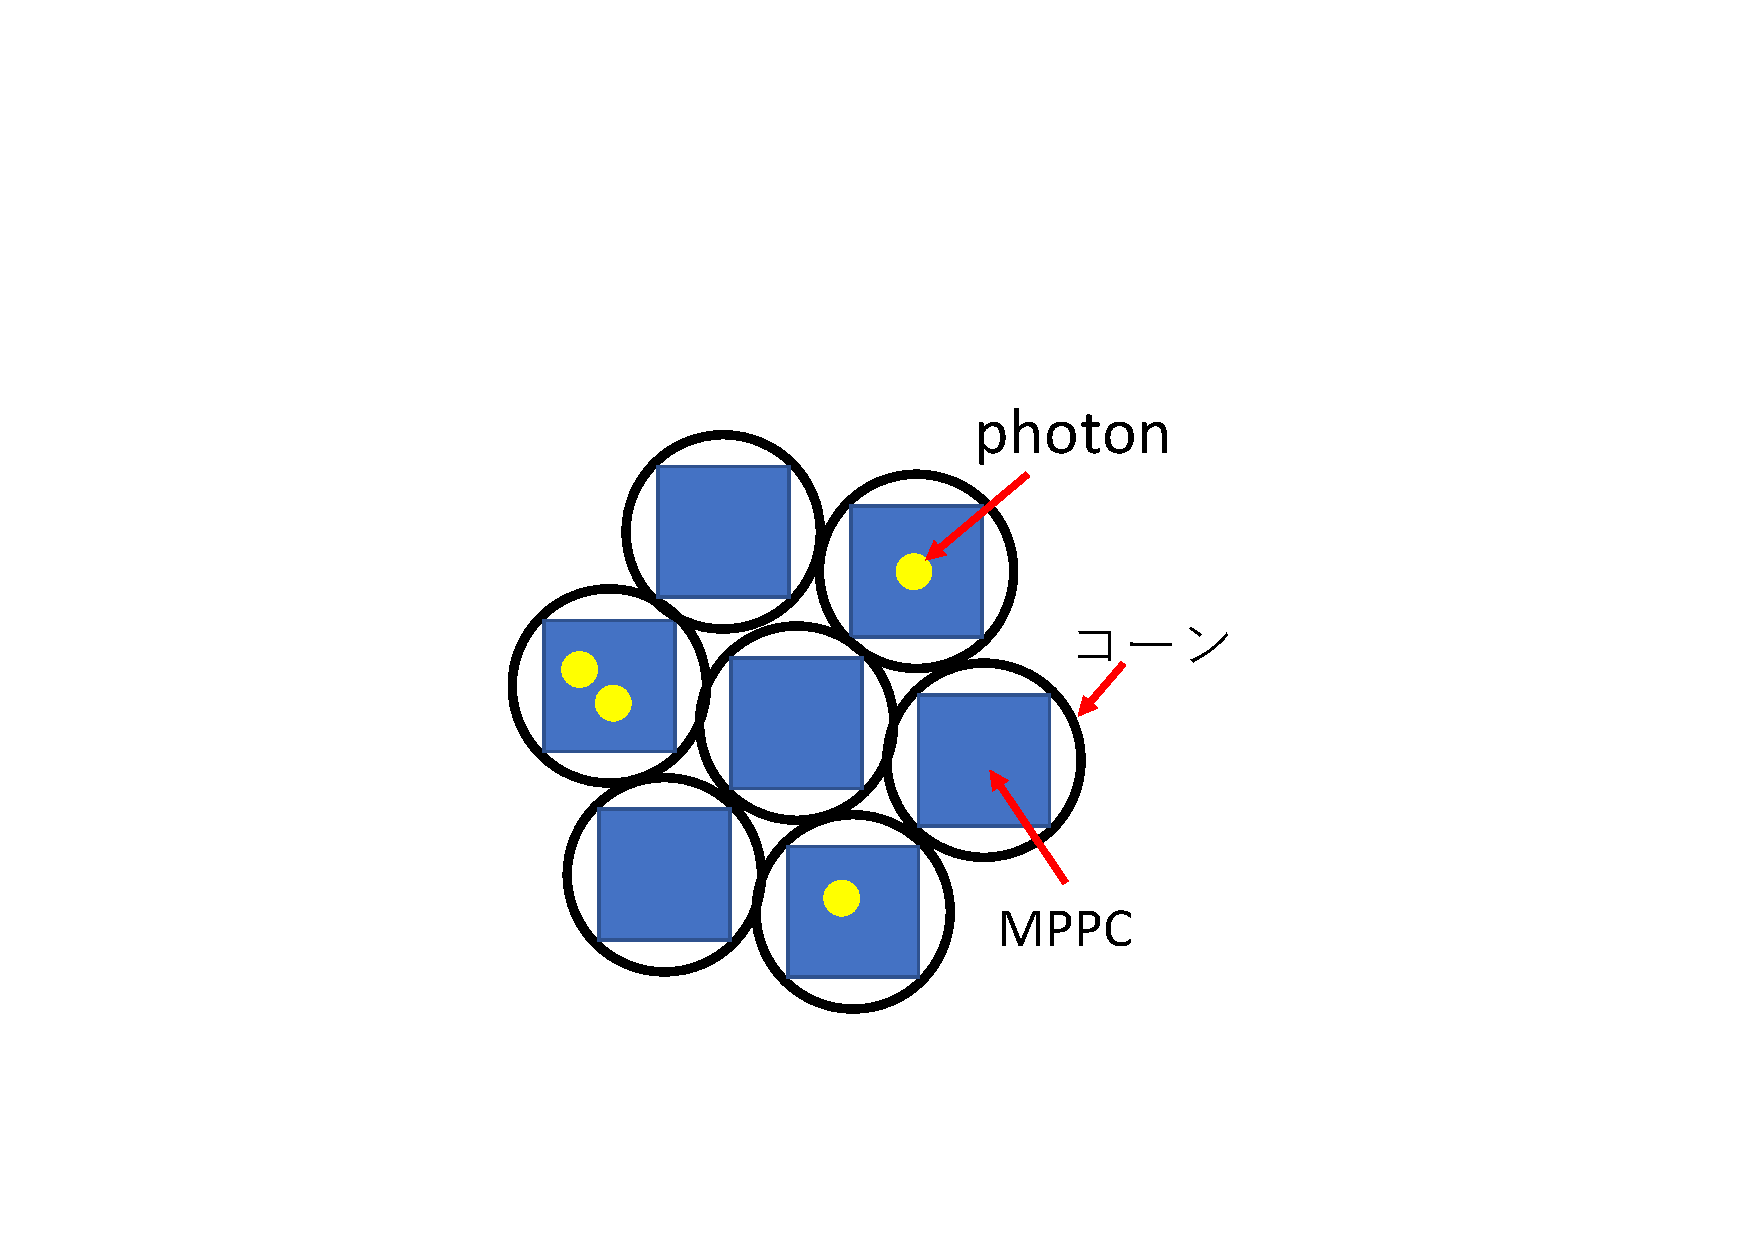
\includegraphics[width=10cm]{images/chapter3/Multiplicity.pdf}
  \caption{Multiplicityの概念図。MultiplicityはPhotonを検出したMPPCの数であるため、この図の場合光子数は4だがMultiplicityは3となる。}
  \label{fig:Multiplicity}
\end{figure}

MPPCに光子が入ったかどうかの判断は、上流のトリガーとのTOFを用いて判断した。
図\ref{fig:TOF}の様に、Peak付近でカットした際のMultiplicityをPeakのMultiplicity、
Peakを外れた$\SI{20}{ns}$以上または以下でカットした際のMultiplicityをDark currentのMultiplicityとした。
また、実際のチェレンコフ光によるMultiplicitySignalを$\rm{Peak} - \rm{Dark current}$として計算した。
その結果を図\ref{fig:Multiplicity_hist}に示す。
Dark currentのMultiplicityは、カット幅に比例していることが分かる。
SignalのMultiplicityは、カット幅$\SI{10}{ns}$付近で増加が緩やかになり、$\SI{20}{ns}$付近でサチュレーションしている。
第4章でのシミュレーションでは、カット幅$\SI{20}{ns}$でサチュレーションしている時のMultiplicityを元に、
コーン型ライトガイドのパラメータを決定した。

\begin{figure}
  \centering
  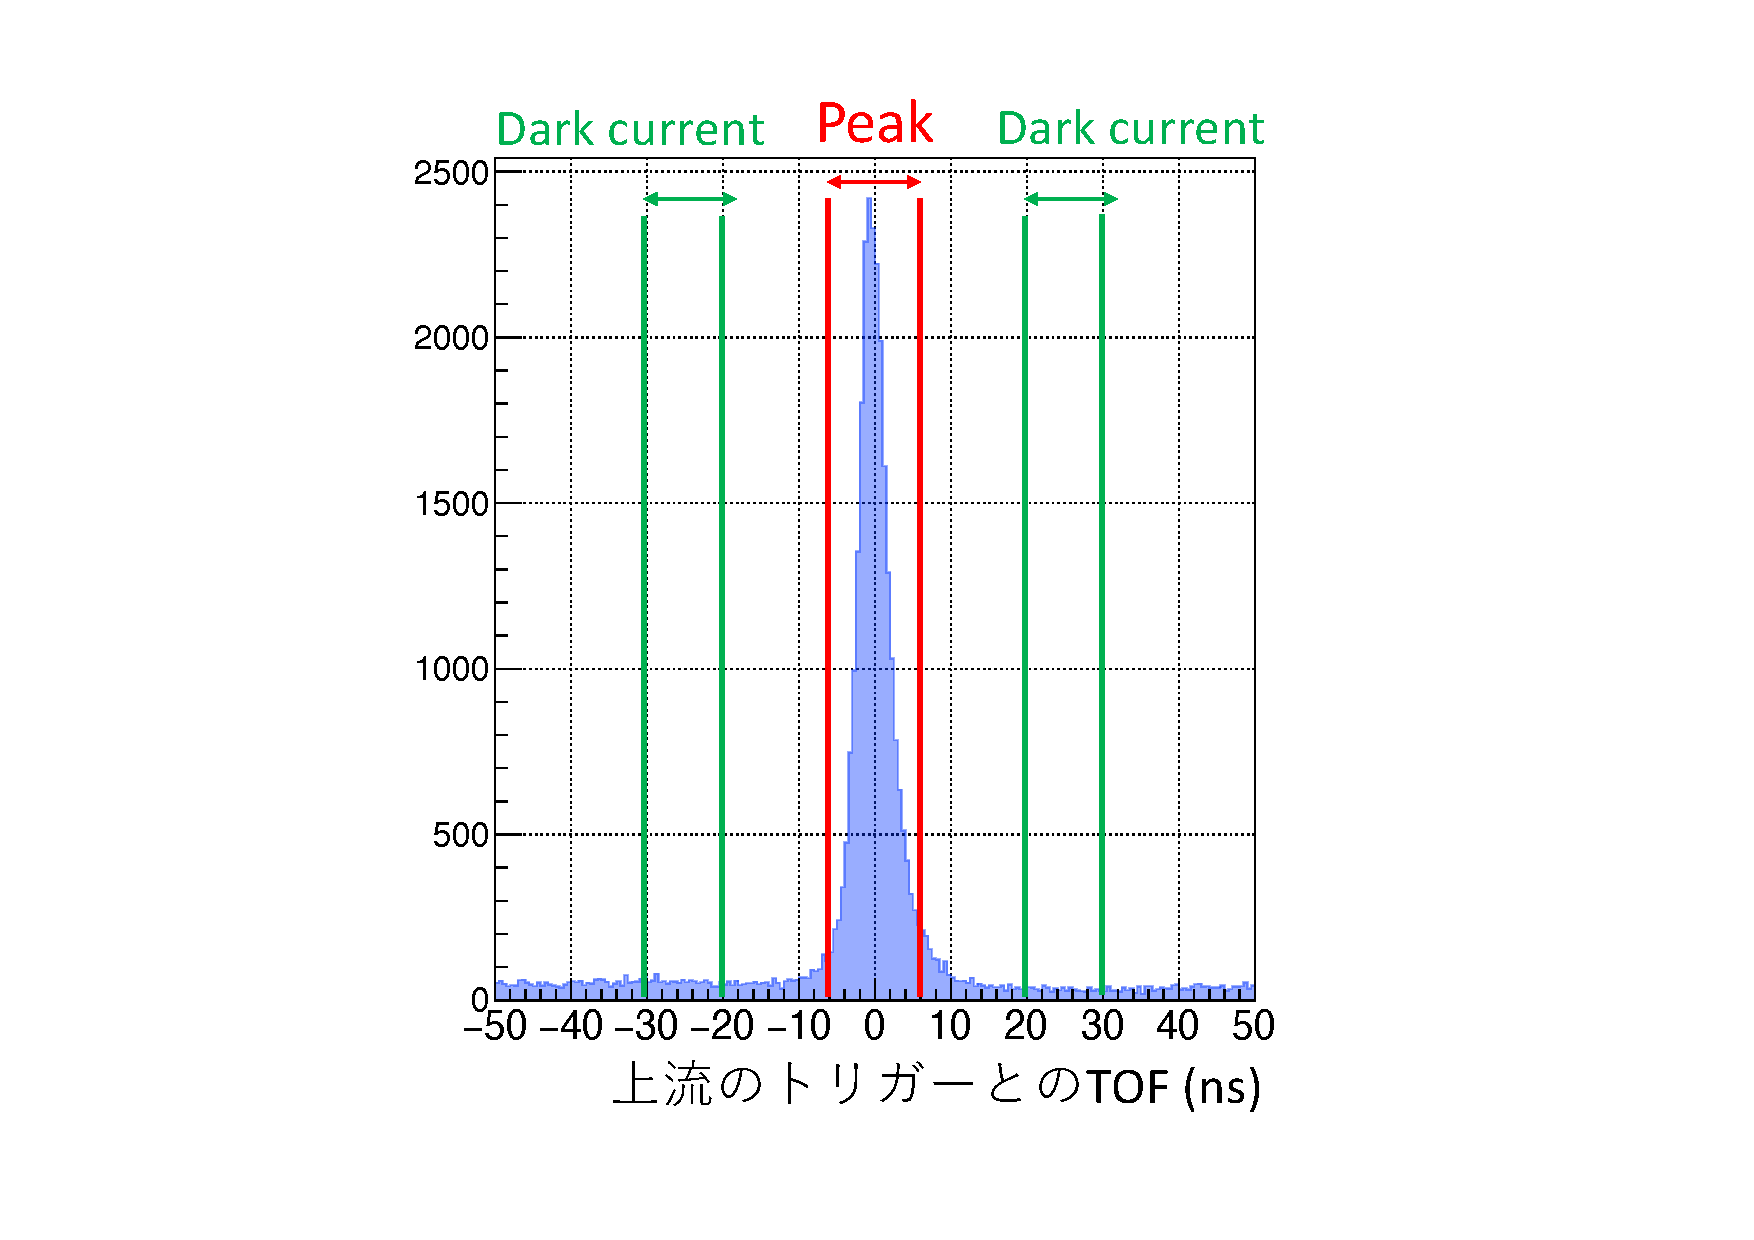
\includegraphics[width=10cm]{images/chapter3/TOF.pdf}
  \caption{MPPCと上流のトリガーとのTOF分布。}
  \label{fig:TOF}
\end{figure}

\begin{figure}
  \begin{tabular}{cc}
    \begin{minipage}[t]{0.45\hsize}
      \centering
      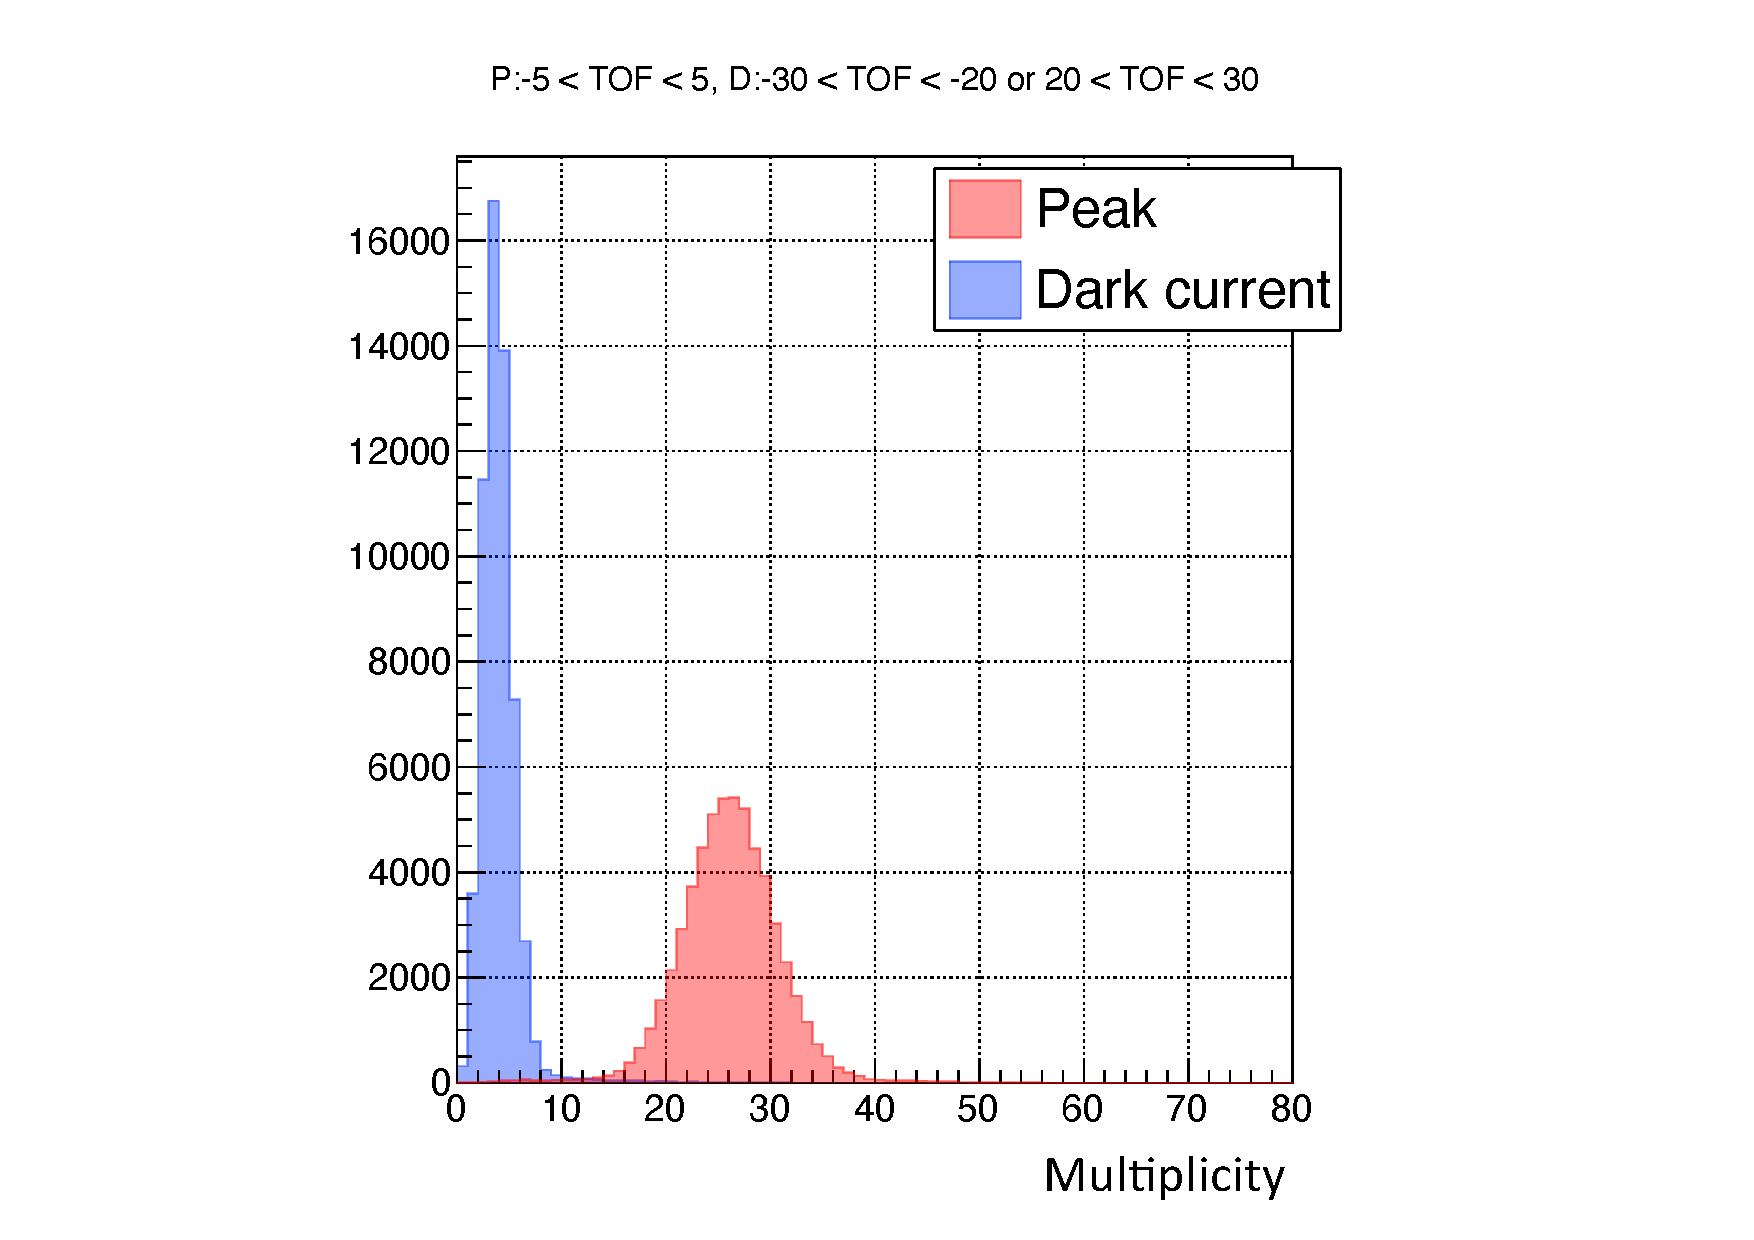
\includegraphics[keepaspectratio, scale=0.3, page=1]{images/chapter3/Analysis3.pdf}
      [a]
    \end{minipage}
    \begin{minipage}[t]{0.45\hsize}
      \centering
      \includegraphics[keepaspectratio, scale=0.3, page=2]{images/chapter3/Analysis3.pdf}
      [b]
    \end{minipage}
  \end{tabular}
  \caption{
  [a]はカット幅$\SI{10}{ns}$の場合のPeakとDark currentのMultiplicity。
  [b]は[a]で得られたMeanをカット幅ごとにプロットしたもの。
  Signalはカット幅$\SI{20}{ns}$あたりでサチュレーションすることが分かる。
  }
  \label{fig:Multiplicity_hist}
\end{figure}

\subsection{Dark currentの評価}
Dark currentは確率的に発生するため、図\ref{fig:TOF}の様にPeakの分布から外れたところでカットをすることで
レートを見積もることができる。
ピークを外したカット幅$\SI{3500}{ns}$でMPPCのDark currentの発生回数を求め、ポアソン分布でフィットを行った。
代表的なCHの分布を図\ref{fig:darkCurrentRate1}に示す。
CH毎にDark currentのレートを評価した。
その結果を図\ref{fig:darkCurrentRate2}に示す。
第4章では、ここで得られたDark currentのレートを考慮したシミュレーションを行った。

\begin{figure}
  \begin{tabular}{cc}
    \begin{minipage}[t]{0.45\hsize}
      \centering
      \includegraphics[keepaspectratio, scale=0.3, page=2]{images/chapter3/darkCurrentRate.pdf}
    \end{minipage}
    &
    \begin{minipage}[t]{0.45\hsize}
      \centering
      \includegraphics[keepaspectratio, scale=0.3, page=3]{images/chapter3/darkCurrentRate.pdf}
    \end{minipage}
  \end{tabular}
  \caption{$\SI{3500}{ns}$幅でカットした際のDark currentの発生回数。ポアソン分布でフィットし、レートを計算した。}
  \label{fig:darkCurrentRate1}
\end{figure}

\begin{figure}
  \centering
  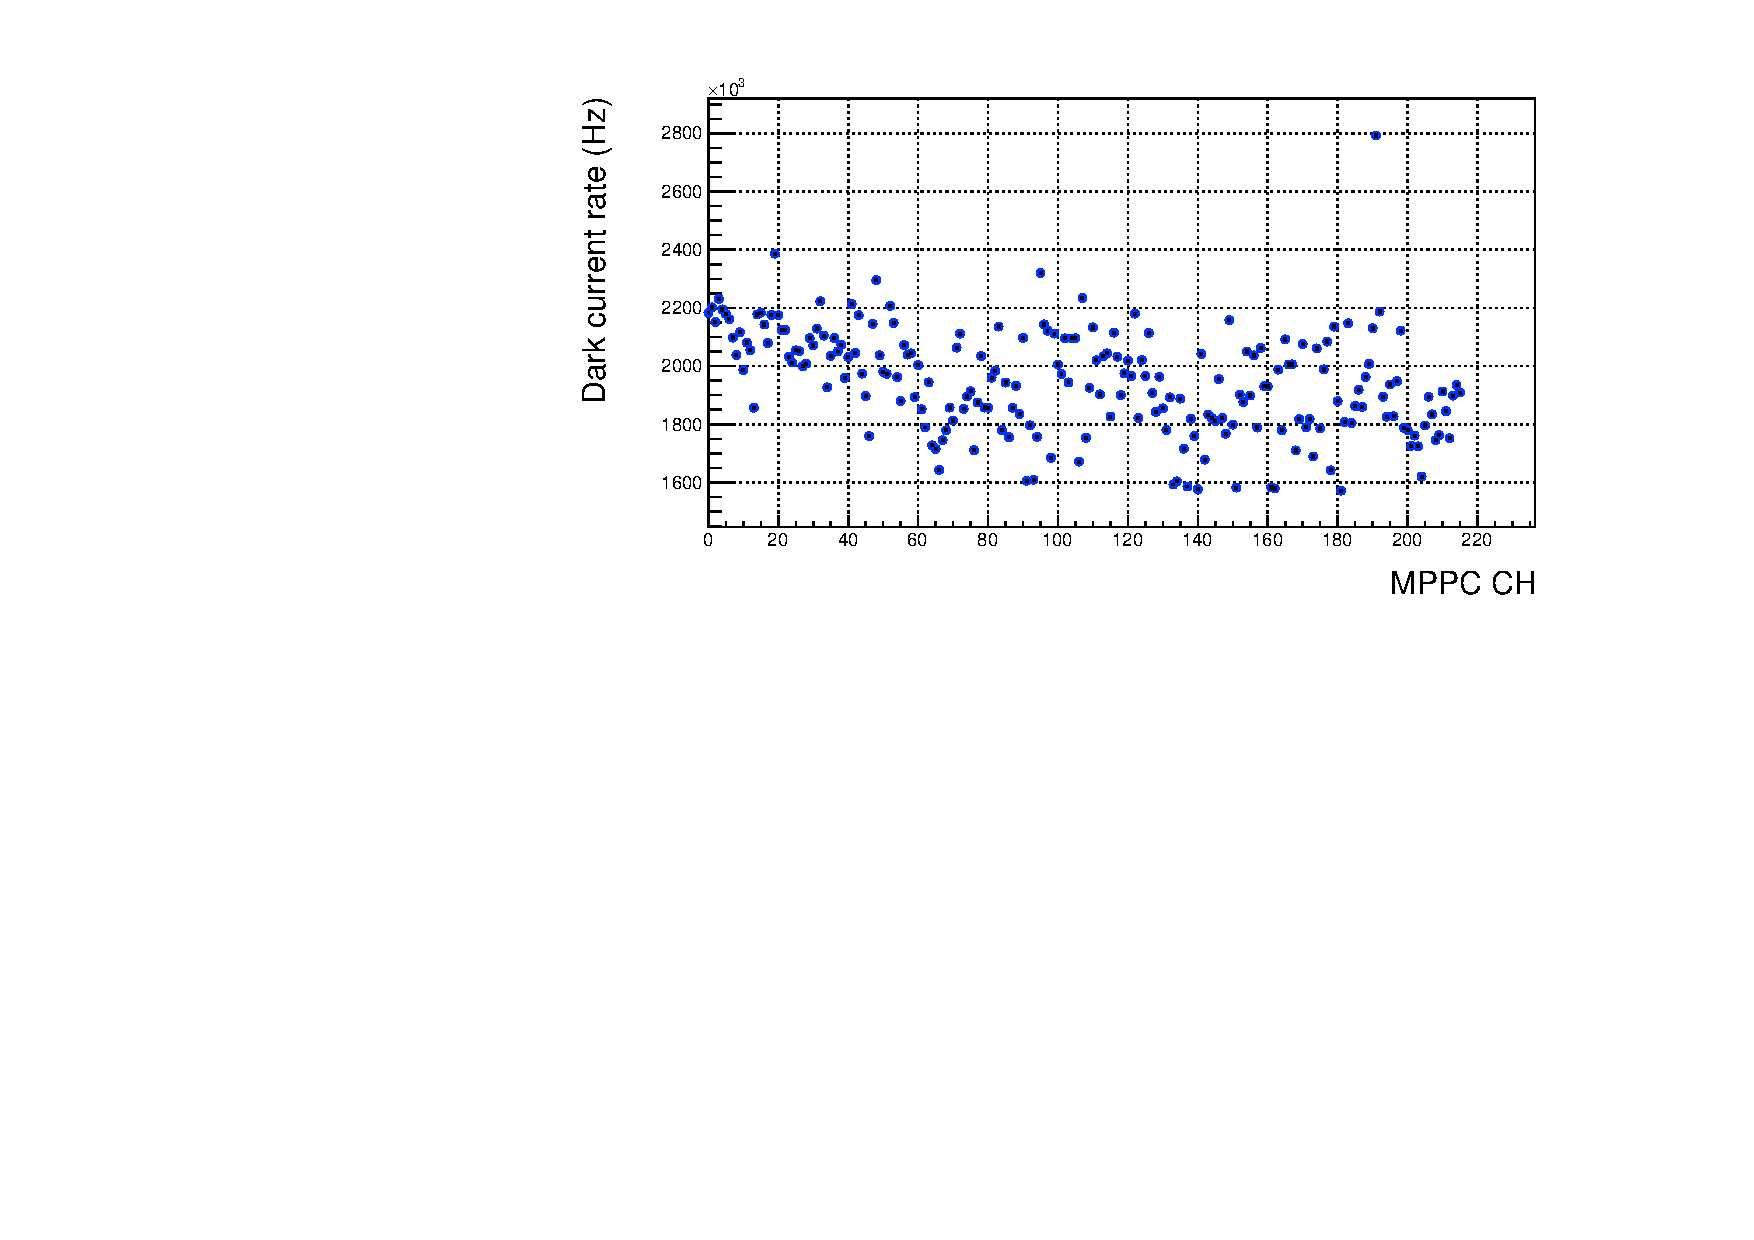
\includegraphics[width=15cm, page=1]{images/chapter3/darkCurrentRate.pdf}
  \caption{$\rm{V_{ov}}$\space$\SI{4}{V}$でのCH毎のDark currentレート。}
  \label{fig:darkCurrentRate2}
\end{figure}